% intro should describe and justify this cahpter
% 
\graphicspath{{chapters/3.Chapter_1/figures}}

\chapter{Endosymbiont Diversity}\label{chap:endo_diversity}

\section{Introduction}

\subsection{Endosymbiont taxonomics}

As briefly discussed in \ref{chap:intro} the taxonomic relations
of the green algae and in particular the Chlorellacea 



\begin{figure}[h]
    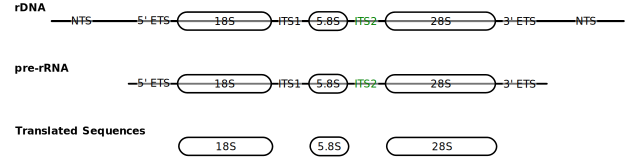
\includegraphics[width=\textwidth]{ITS_schematic.pdf}
    \caption{Structure of Eukaryotic nuclear ribosomal DNA.
        rRNA genes exist in tandem repeats separated by nontranscribed spacers (NTS).
        pre-rRNA contain 
    Redrawn from \citep{}}
    \label{fig;its2_schematic]}
\end{figure}



Algal is a clusterfuck

The nuclear ribosomal internal transcribed spacer 2 (ITS2) is a well used


ITS2 has shown particular utility in the identification and separation
of closely related green algal species \citep{Buchheim2011}.


However, this type of barcoding approach to species identification is 
imperfect 



Species concepts  - ITS2 vs 18S vs whatever \citep{Boenigk2012}

\subsection{Clonality of endosymbionts}

Single cell genomes






\subsection{Elimination of endosymbionts}



Clearing endosymbiont - paraquat \citep{Hosoya1995a}, dark \citep{Karakashian1963}, DCMU german paper \citep{Reisser1976},
X-ray \citep{Wichterman1948}, cyclohexamide \citep{Weis1984,Kodama2007}


Paraquate Hosoya 
Kodama


Fortunately, to this end, the only other published 2nd generation sequencing analysis of \textit{P. bursaria} and a green algal,
endosymbiont: Kodama \textit{et. al.} 2014 \citep{Kodama2014} partially addressed this issue.  This analysis investigated 
the differential global metatranscriptome profile of \textit{P. bursaria} Yad1g strain with and without its \textit{Chlorella variabilis} 1N endosymbiont 
\citep{Kodama2014}.   While, this is a different strain of both host and endosymbiont to the CCAP1660/12 strains (\textit{P. bursaria} and \textit{Micractinium reisseri}) 
used in this thesis it offers a potential avenue to investigate these other components.


An attempt was made to replicate this work using the CCAP1660/12 strains, unfortunately, elimination of the endosymbionts without death of the host
didn't prove possible in these strains.  Despite using 
(despite earlier publications to the contrary) by either maintaining the culture in the dark \citep{Siegel1960} (although some studies have thrown doubt on
        how effective this method is at completely elimiating the photobiont \citep{Tanaka2002}) or treatment with various titrations of herbicides 
            (e.g. paraquat \citep{Hosoya1995a}) or the protein synthesis inhibitor cyclohexamide \citep{weis1984effect}).\footnote{
        There are naturally aposymbiotic strains of \textit{Paramecium bursaria} \citep{Tonooka2002a}}






\section{Aim}

In this chapter I will determine the exact algal endosymbiont strains present
in the 3 principal \textit{Paramecium bursaria} cultures used throughout
this thesis and their relationships relative to one another and to
other green algae.

I will also use single cell genomics to investigate whether the algal
endosymbiont present in the \textit{Paramecium bursaria-Micractinium reisseri}
CCAP 1660/12 strains form a clonal population. 

Finally, I will discuss the attempts to remove the endosymbiont in the 
\textit{Paramecium bursaria} CCAP 1660/12 strain from the host.


\section{Methods}

\subsection{Taxonomic Investigation}
    
\subsubsection{ITS2 Sequencing}

\textit{Paramecium bursaria} CCAP 1660/12 and \textit{Paramecium bursaria} CCAP 
1660/13 cultures were maintained in New Cereal Life (NCL) media
at \(18\celsius\) with 12:12 hour light/dark cycle.

ITS2 sequences were amplified from 3 separate biological replicates 




ITS2 sequences were amplified using ITS2-S2F and CHsp prime


\textit{Paramecium bursaria} 1660/13 ``Coccomyxa'' 
1k-10k used ITS2-S2F and ITS4-R
1D-3D using ITS2-S2F and CHsp
i


PCR products were then cleaned up, cloned, sequenced
and processed using the same protocol as \citep{Maguire2014a}.

Briefly, the successfully amplified PCR products were gel-purified 
(Wizard SV Gel and PCR Clean-Up kit, Promega).
These products were then TA-cloned 
using Agilent's PCR StrataClone Cloning Kit in a PSC-A-amp/kan
vector.
Successful clones were blue-white screened and 5 clones
selected for each PCR product.  
Clones were then externally Sanger sequenced using the M13Rev primer
at MWG Eurofins. 








Flanking vector and primer sequences were removed: sequenced trimmed to 
areas of high chromatograph quality and ambiguously defined bases corrected
using Sequencher \citep{Sequencher}.


From the 3 \textit{Paramecium bursaria} CCAP 1660/12 biological replicates
14, 9, and 11 ITS2 sequences were obtained respectively.





In order to mitigate the risk of sequencing error masquerading
as true sequence divergene any sequences found in later phylogenetic
analysis to demonstrate single nucleotide changes from the consensus
of its clade placement was resequenced at MWG Eurofins in reverse 
using M13Uni.  Specifically, these were ITS-B18,
ITS-2, ITS-19, ITS-B6, ITS-B3, ITS-A7, ITS-6, ITS-B15,
ITS-10, ITS-9, ITS-15, and ITS-1.
If the reverse sequencing didn't demonstrate the same polymorphism as
the original forward sequencing it was considered to be a likely 
sequencing error artefact and the divergent sequence was removed. 

%<> examples

\subsubsection{18S Sequence determination}

All assembled transcriptome contigs were BLASTP 
against all Chlorella 18S sequenced from 
\citep{Imamura2008}.



ITS2 sequences used in \citep{Hoshina2010}, \citep{Hoshina2013} were retrieved
from genbank



\subsubsection{Phylogenetics}

Sequences were 





\subsection{Single Cell Genomics}

\subsubsection{DNA Extraction}

\subsubsection{Library Preparation}

\subsubsection{Illumina Sequencing}

\subsubsection{Read pre-processing}

Trimmomatic was used to trim sequencing adapters (using sequences
provided by Exeter Sequencing Service).
Reads were then quality trimmed at both a minimum average sliding window
quality threshold of Q5 and Q30. 

Additionally, reads were error corrected using Bayeshammer incorporated into 
the Spades assembler. 

\subsubsection{Assembly}

Assemblies of Q5 and Q30 trimmed reads were conducted using
the Spades assembler, Megahit, and Platanus. 
Spades was run with and without autocov thresh
Megahit was also run on spades corrected Q30 trimmed reads. 

\subsubsection{Comparative Analysis}

Assemblies were compared using QUAST.





Contigs were subsequently cut into 10kb fragments for consistency
in binning and taxonomic assignment.
Reads were mapped back onto the final assembly using Bowtie2 
\citep{Langmead2012} 

Using the metagenomic binning tool, CONCOCT \citep{Alneberg2014}
contigs were binned into clusters based on sequence composition
and coverage features (derived from mapping data).
Coverage features were derived from a coverage and linkage table
generated via CONCOCT scripts built around BEDTools \citep{Quinlan2010,Quinlan2014}, Picard \url{http://broadinstitute.github.io/picard/} 
and Samtools \citep{Li2009} 
based parsing
of the bowtie2 alignment files.

Clustering was conducted using a Gaussian Mixture Model (GMM) \citep{Bishop2006}
and the number of clusters determined through variational Bayesian inference \citep{Corduneanu2001}.

All CONCOCT analyses were completed using a provided pre-configured 
Docker Image \citep{Merkel2014}, a form of lightweight 
distributable process isolation container.
This was downloaded from DockerHub \url{https://hub.docker.com/r/binpro/concoct/}
on 2015-10-25.



Additionally, the cut contigs were taxonomically assigned 
using TAXAssign \url{https://github.com/umerijaz/TAXAassign} against the NCBI nt database. 

The BLAST database was downloaded using update\_blastdb.pl script \url{http://www.ncbi.nlm.nih.gov/blast/docs/update_blastdb.pl}
and TAXAssign was run in parallel (using GNU parallel \citep{Tange2011a})
with a maximum of 10 reference matches
per contig a minimum percentage identity for assignment
to a given taxonomic level of 60, 70, 80, 95, 95, and 97
for Phylum, Class, Order, Family, Genus and Species respectively. 


CONCOCT clusters were then evaluated using the taxonomic assignments from TAXAssign
using the provided ``validate.pl'' script.




\subsection{Endosymbiont elimination}

\subsubsection{Paraquat}

\subsubsection{Cyclohexamide}

\subsubsection{Darkness}




\section{Results}

\subsection{ITS2 Phylogeny}



\subsection{18S Fragment Phylogeny}

All assembled contigs from final transcriptome assembly (see \ref{chap:})


\subsection{Assembly}

\subsubsection{Binning}

CONCOCT

\begin{figure}
	\includegraphics[width=\textwidth]{CONCOCT_clusters.pdf}
	\caption{A low dimensional Principal Component representation of genomic contig
		cluster assignments.  Clusters are assigned via a Gaussian Mixture Model (GMM) 
		based on sequence compositional and coverage features as implemented in CONCOCT.
		Unfortunately, as can be observed clusters are both poorly distinguished even
		in the dimensions of the 2 principal components (PCA1 and PCA2) and are numerous (34). 
	\label{fig:concoct_clusters}
\end{figure}


TAXAssign assigned 3,037 labels to the 11,757 contigs. 
\begin{table}
	\begin{tabular}{r | l c |}
\textbf{Source Group} & \textbf{Number of Contigs} & \textbf{Phylum-Level Breakdown} \\
\hline
\textbf{Host} & 13 & Intramacronucleata\\
- & 2  & Apicomplexa\\
- & 1  & Colponemidia \\
\hline 
\textbf{Endosymbiont} & 12 & Chlorophyta\\
- &  12 & Streptophyta\\
- &  1 & Cyanobacteria\\
\hline
\textbf{Bacterial Contamination} & 16230 & Proteobacteria \\
- & 468 & Firmicutes\\
- & 329 & Actinobacteria\\
- & 128 & Bacteroidetes/Chlorobi group\\
- & 1 & Deinococcus-Thermus\\
\hline
\textbf{Eukaryotic Contamination} & 605 & Ascomycota \\
 - & 380 & Chordata\\
 - & 74 & Arthropoda \\
 - & 12 & Basidiomycota\\
- & 7  & Nematoda \\
- & 1 & Platyhelminthes\\
- & 1 & Cnidaria\\
\hline
\textbf{Unknown} & 540 & Unclassified \\
\hline
	\end{tabular}
	\caption{Summary of taxonomic assignments via TAXAassign grouped into putative ``source groups'' reflecting
		the most probable source of 10kb chunked contigs of that specific taxonomic provenance.  Of note, is the disproportionate
		number of contigs from contaminating sources. Specifically, }
	\label{}
\end{table}


    

Clusters were additionally validated by comparison to taxonomically BLASTN
assigned contig labels.    



11,757 contigs with 3,3037 were clustered into 34 unique clusters.
When these clusters were compared with a ``ground-truth'' from
the taxonomic assignment of clusters 

\begin{table}
	\begin{tabular}{| c || c | c |}
		 - & Positive & Negative \\
		 \hline
		 \hline
		True  &  Contigs with same taxonomic assignment are assigned to the same cluster  & Contigs with different taxonomic assignments are assigned to different clusters\\
		False &  Contigs with different taxonomic assignments are assigned to the same cluster  & Contigs with the same taxonomic assignment are assigned to different clusters \\
	\end{tabular}
	\caption{A contextual explanation of True and False Positive and Negatives in the context of contig binning/clustering.  Top left indicates what a
		True Positive (TP) means in this context, bottom left a False Positive (FP).  Similarly Top Right explains a True Negative (TN) and Bottom Right a
		False Negative (FN)}
	\label{tab:cluster_outcome_explanation}
\end{table}


Recall that Precision and Recall can be defined as follows:
\[Precision = \frac{TP){TP+FP}
Recall=\frac{TP}{TP+FN}\] 
where \(TP\) are True Positives and \(FP\) and \(FN\) are False Positives
and Negatives respectively (see \cref{tab:cluster_outcome_explanation} for an 
explanation of what these terms mean in the context of clustering).

CONCOCT assigned clusters were relatively precise \(0.912608\) 
therefore there were relatively few \(FP\) i.e. the majority of clusters 
contained contigs with the same taxonomic assignments. 

However, recall was relatively poor \(0.542250\) suggesting a
fair number of FN i.e. contigs with the same taxonomic assignments
were not confined to a single cluster and were spread over main clusters.

The \(F_1\)\footnote{\(F_1 = 2 * \frac{precision * recall)}{[precision + recall]}\)} score for CONCOCT 
clustering was therefore \(0.680389\) under the, slightly flawed, assumption that 
TAXAssign represents the ground-truth.

It is also worth noting that the 34 clusters had a relatively high level of mutual information
(Normalised Mutual Information of \(0.332022\) and a Rand Index of \(0.499741\)) suggesting
many small but highly similar clusters were created.  This level of similarity combined
with the poor recall suggests a greater number of clusters were necessarily present in the
ground-truth.

\subsection{Elimination}
\subsubsection{Paraquat}
\subsubsection{Cyclohexamide}
\subsubsection{Darkness}





\section{Discussion}

\subsection{Reliability of Culture Collection}

The clear result is that despite the \textit{Paramecium bursaria} CCAP 1660/13
supposedly containing a \textit{Coccomyxa} endosymbiont 
all ITS2 sequences from this culture differeed fromt he published
\textit{Coccomyxa} sequence (accession \(AB260896.1\)) and were identical
to those sequences from the \textit{Paramecium bursaria} CCAP 1660/12 \textit{Micractinium
reisseri} endosymbiont.



Unfortunately, on communication with CCAP it emerged that they lost
the CCAP 1660/11 and 1660/12 strains in their collection. 


CCAP 1660/13 had become overgrown by free-living \textit{Coccomyxa}. 

However, it emerged that despite previous findings that CCAP 1660/13
did appear to contain the \textit{Coccomyxa} by \citep{Imamura2008} this was
likely to be contamination from the \textit{Coccomyxa} in the media as 
the CCAP 1660/12 and CCAP 1660/13 cultures were isolated from the same
pond (Cambridge, UK) by CCAP and appear to both have \textit{Micractinium
reisseri} endosymbionts.

This was confirmed by our ITS2 analysis.


However, this all demonstrates clear evidence of not taking previous studies
or culture collection descriptions without careful consideration.





taxonomic resolution - barcoding?
ITS2 sequencing could be improvied - possible sequencing erroA/r 


\subsection{Clonality of endosymbionts}



\subsection{Diversity of traits in endosymbionts}



\section{Conclusions}

Despite over 50 identified strains 


Is the endosymbiont clonal?
ITS2 - yes it is
18S - why are we getting these fragments but kind of yes

Is it the species we think it is?
Yes 18S/ITS2 among green algae


file:///home/fin/Downloads/AiM20120300003_34647180.pdf
gt





Potentially, we are faced with the possibility that metabolic co-dependence has become fixed in 1660/12
relative to the YADGN1 strain of Kodama.


